\documentclass{article}
\usepackage[backend=biber, style=authoryear, sorting=nyt, style=numeric]{biblatex}
\usepackage{url}
\usepackage[dvipsnames]{xcolor}
\usepackage{enumitem}

\usepackage{background}
\usepackage{tikz}
\usepackage{geometry}
\usetikzlibrary{shapes, arrows, positioning}
\usepackage[T1]{fontenc}
\usepackage[utf8]{inputenc}
\usepackage[british]{babel}
\usepackage{titletoc}
\usepackage{titlesec}
\usepackage{lipsum}
\usepackage{tocloft}
\usepackage{hyperref}
\usepackage{algorithm}
\usepackage{algpseudocode}
\usepackage{graphicx}
\usepackage[section]{placeins}
\usepackage{caption}
\usepackage{textcomp}
\usepackage{subcaption}
\usepackage[edges]{forest}
%\usepackage[superscript,biblabel]{cite}
\usepackage{fontawesome5}
\usepackage{algorithm}
\usepackage{algpseudocode}
\usepackage{amsmath}
\usepackage[simplified]{pgf-umlcd}
\usepackage{enumitem}
\usepackage{adjustbox}
\usepackage{listings}
\usetikzlibrary{shapes.geometric, arrows}
%\usepackage[style=ext-authoryear, backend=biber]{biblatex}
%\usepackage{url}
%\usepackage[style=authoryear]{biblatex}
\addbibresource{rapport.bib}
%\usepackage{cite}
\usepackage[british]{datetime2} % Enhanced date and time.

\addbibresource{rapport.bib}

\definecolor{aerospaceblue}{RGB}{0, 128, 255} % Couleur bleu ciel pour l'aérospatiale
\definecolor{myblue}{RGB}{0, 0, 255}

% Define the theme colors
\definecolor{blue}{RGB}{0,0,255}
\definecolor{green}{RGB}{0,128,0}
\definecolor{red}{RGB}{255,0,0}
\definecolor{custompurple}{RGB}{128,0,128}

% Set the lstset configuration
\lstset{
	language=C++,
	basicstyle=\ttfamily\small,
	keywordstyle=[1]\color{blue},
	keywordstyle=[2]\color{black},
	keywordstyle=[3]\color{green!60!black},
	commentstyle=\color{green!60!black},
	stringstyle=\color{red},
	otherkeywords={CALL},
	morekeywords=[1]{CALL},
	morekeywords=[2]{FOPENSUBNODES},
	numbers=left,
	numberstyle=\tiny,
	stepnumber=1,
	numbersep=5pt,
	frame=single,
	breaklines=true,
	breakatwhitespace=true,
	tabsize=4,
	captionpos=b,
	showstringspaces=false,
	% Adjust the frame margins for a larger rectangle
	xleftmargin=1em,
	framexleftmargin=1em,
	framexrightmargin=1em
}


\tikzset{
	startstop/.style={
		rectangle,
		rounded corners,
		minimum width=3cm,
		minimum height=1cm,
		text centered,
		draw=black,
		fill=red!30
	},
	io/.style={
		trapezium,
		trapezium stretches=true, % A later addition
		trapezium left angle=70,
		trapezium right angle=110,
		minimum width=3cm,
		minimum height=1cm,
		text centered,
		draw=black,
		fill=blue!30
	},
	process/.style={
		rectangle,
		minimum width=3cm,
		minimum height=1cm,
		text centered,
		text width=3cm,
		draw=black,
		fill=orange!30
	},
	decision/.style={
		diamond,
		minimum width=3cm,
		minimum height=1cm,
		text centered,
		draw=black,
		fill=green!30
	},
	arrow/.style={
		thick,
		->,
		>=stealth
	}
}

\newcommand{\coloredsquare}[1]{\textcolor{#1}{\rule{1em}{1em}}}

\renewcommand{\cfttoctitlefont}{\hfill\large\bfseries\fontsize{20}{24}\selectfont}
\renewcommand{\cftaftertoctitle}{\hfill\mbox{}}

\definecolor{mydarkyellow}{HTML}{87CEEB}
\definecolor{lightblue}{RGB}{173,216,230}
\definecolor{lightyellow}{RGB}{255,255,204}
\definecolor{yellow}{RGB}{255,255,0}

\backgroundsetup{
	scale=1,
	color=black,
	opacity=0.5,
	angle=0,
	contents={
		\ifnum\value{page}=1
		\begin{tikzpicture}[remember picture,overlay]
			\path [fill=mydarkyellow] (current page.south west) rectangle (current page.north east);
		\end{tikzpicture}
		\fi
	}
}

\title{\textbf{\Huge Project Report}\\[1cm]
	\textbf{\LARGE Polytech Nice}\\[2cm]
	\hrule height 1pt
	\vspace{0.5cm}
	\textbf{\Large Simple Road Traffic Modeling}\\[0.5cm]
	\hrule height 1pt
	\vspace{3cm}
	\small{\today{}}}

\author{
	\begin{tabular}{c}
		Gerbaud Florent \\ Fatima Rharrour \\ \\
		9-th october to 20-th December september 2023\\
		\\ Academic tutor : Didier Auroux
	\end{tabular}
}

\date{}
\begin{document}
	\maketitle
	\hspace{2cm}
	\begin{figure}[b]
		\centering
		\begin{minipage}[b]{0.45\linewidth}
			
\includegraphics[width=5cm]{logo.png} \\
			%Company tutor : Vincent Vadez
		\end{minipage}
		\hfill
		\begin{minipage}[b]{0.45\linewidth}
			\raggedleft
			\vspace{-0.5cm}
			
\includegraphics[width=6cm]{Polytech.png} \\
			%Academic tutor : Cédric Boulbe
		\end{minipage}
	\end{figure}
	\newpage % ajout d'un saut de page
	% Table des matières
	\renewcommand{\contentsname}{
		\hfill
		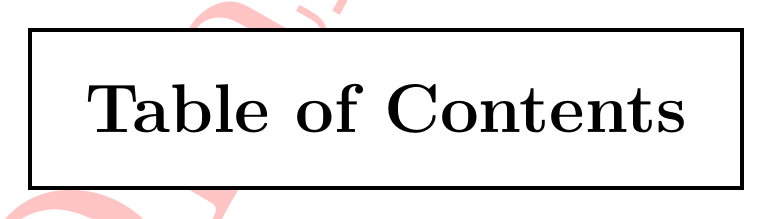
\begin{tikzpicture}
			\node[draw, fill=white, inner sep=20pt,line width=1.5pt] {\fontsize{30}{36}\selectfont\bfseries Table of Contents};
		\end{tikzpicture}
		\hfill
	}
	\tableofcontents
	\newpage
	\listoffigures % Add a listing of figures
	
	\listofalgorithms
	\newpage
	\section{Presentation of the Subject}
	\subsection{Useful Definition}
		\textbf{\underline{Ordinary Differential Equation (ODE):}} \newline\newline
		An ODE is a mathematical equation that relates a function to its derivatives with respect to one or more independent variables. ODEs are commonly represented given a function F of x, y, and derivatives of y. Then, an equation of the form
		\begin{align*}
			F\left(x,y,y',\ldots ,y^{(n-1)}\right)=y^{(n)}
		\end{align*}
		
		\textbf{\underline{SMRT}} 
		SMRT means Simple road traffic simulation \newline\newline
		\textbf{\underline{microscopic simulation}} 
		
		Microscopic simulation is a computer-based modeling technique that simulates the behavior of individual entities, such as vehicles or pedestrians, within a system. It focuses on detailed modeling of each entity's movements, interactions, and behaviors to understand and predict the dynamics of a larger system, like traffic flow or crowd movement. \newline\newline
		
		\textbf{\underline{Macroscopic simulation}} 
		
		Macroscopic simulation models systems at a higher, aggregated level, considering overall behaviors like traffic flow without detailing individual movements. It helps analyze system-level trends and capacities, useful for broader planning.
		
		The relation between microscopic and macroscopic simulation lies in their approach to studying systems. Microscopic simulation focuses on individual entities' detailed behaviors, while macroscopic simulation analyzes aggregated behaviors of the entire system without considering individual entities. They complement each other: microscopic for detailed insights into individual behaviors, and macroscopic for understanding overall system trends and capacities. \newline\newline
		
		If you are interested by these types of modelisation i suggest you to going to see this article \cite{dugois:tel-01505473}
	
	\subsection{Simple Road Traffic Modeling}
	
		Road traffic modeling involves studying how vehicles behave on road networks, with the aim of simulating and analyzing aspects such as traffic flow, congestion, and driver behavior. This field employs mathematical and computer models to understand and predict traffic patterns, playing a crucial role in urban planning, traffic management, and the development of intelligent transportation systems (as shown in Figure \ref{fig:intro}). 
		
		Explore the integration of a driving simulator with a traffic simulator in Jeihani et al.'s study \cite{JEIHANI2017164}, revealing enhanced traffic density and Variable Message Sign (VMS) reliability. The findings suggest that integration positively influences compliance behavior and factors affecting route diversion.
		
		
		\begin{figure}[H]
			\centering
			\includegraphics[width=0.8\textwidth]{intro.jpg}
			\caption{\textbf{\underline{Road Traffic:}} An illustrative example of a road traffic phenomenon, which is the focus of our study.}
			\label{fig:intro}
		\end{figure}
	
		
		\subsubsection{The Objective of SMRT}
		The primary goal of simple road simulation is to analyze and understand vehicle behavior in a controlled and reproducible environment. Researchers and engineers use these simulations to study the impact of various factors on traffic flow, safety, and efficiency. This contributes to the development and testing of traffic management strategies and vehicle control systems, providing insights into the dynamic interactions between vehicles and the road environment.
		
		\subsubsection{Use Case to Explain the Interest of These Simulations}
		Simple road simulations find applications in various fields, including urban planning, transportation engineering, and autonomous vehicle development. For instance, they can assess the effectiveness of new traffic signal timings, study the implications of road design changes, or test the performance of autonomous vehicles in different traffic scenarios. These simulations offer a cost-effective and risk-free way to evaluate real-world interventions and innovations, enhancing decision-making processes and supporting the development of sustainable and efficient transportation systems.
		
		\subsubsection{Field of Application}
		Simple road simulation is applied across a wide range of fields, including transportation research, traffic engineering, and urban planning. It plays a crucial role in the development and validation of autonomous vehicle technologies. The ability to model and simulate various road conditions helps researchers and practitioners make informed decisions, improving the design and management of transportation systems. Simple road simulation serves as a powerful tool for enhancing our understanding of traffic dynamics and contributes to the ongoing evolution of smart and adaptive transportation systems.
		
	
	\subsubsection{Using GitHub for Project Management}
	In this project, we selected GitHub as the primary management tool to facilitate our collaboration, track changes, and manage the source code. The following representation provides an overview of our collaborative use of GitHub as a pair throughout the project.
	\begin{figure}[H]
		\centering
		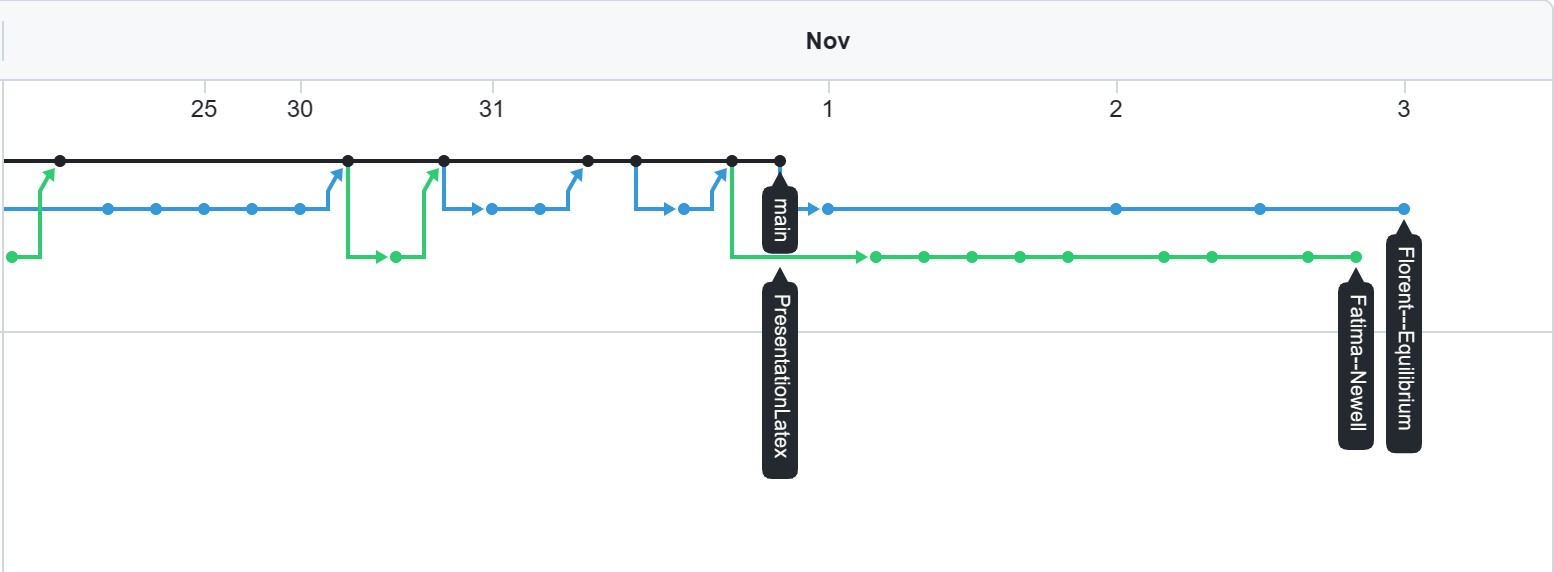
\includegraphics[width=0.8\textwidth]{GitHub.jpg}
		\caption{\textbf{\underline{Road traffic : }} In this picture, you can see an example of a road traffic phenomenon that we could study}
		\label{fig:GitHub}
	\end{figure}
	
	\section{Project Objectives}
	
	This project could be decomposed into different parts. The primary objectives of the project were to conduct microscopic and macroscopic simulations.
	
	\subsection{Microscopic Simulation}
	
	
	In the case of microscopic simulation, the objective was to simulate traffic flow phenomena using two types of models.
	The first model was a linear approach that considered only the position of the car in front of it. This model, known as the 'Follow-the-Leader' model, simplistically replicates vehicle behavior by focusing solely on its proximity to the preceding car. It assumes that each vehicle adjusts its speed to maintain a safe following distance.
	
	The second model employed was Newell's method, which is more intricate and offers greater realism. Newell's model considers not only the preceding vehicle's position but also incorporates the speed and acceleration of adjacent vehicles. This method captures the interactions between neighboring cars, resulting in a more nuanced representation of traffic dynamics.
	
	In this modeling, we will focus on the position and velocity of multiple vehicles following each other in a single lane. We will assume that vehicles accelerate when they have open space, maintain their speed when they are close to the vehicle in front, and brake more strongly as they get very close. We will arrange two and then three vehicles, one behind the other, with the first vehicle maintaining a constant velocity, and observe the behavior of the following vehicles.
	Once we done these simulations we are going to add conditions and behaviour a little bit different.
	
	\subsection{Macroscopic Simuation}
	
	In the second part of the project, we encountered the limitations of the Microscopic Model. We will delve deeper into these limitations shortly. In essence, it lacks realism and provides fewer details compared to the macroscopic simulation.
	
	To address this issue, we chose to employ Partial Differential Equations (PDEs). In this type of simulation, we do not solely focus on individual car behaviors but rather treat traffic as a fluid-like entity. This approach allows us to gain a better understanding of traffic flow simulation. Considering traffic as a fluid is justified by its collective behavior resembling fluid dynamics—vehicles move in a continuous flow, similar to how fluids move in pipes or channels. Thus, employing PDEs assists in capturing the overall flow dynamics.
	
	Consequently, we utilize a simplified form of the Navier-Stokes equation to tackle the problem.
	
	This enables us to refine our description of the previous simulations by providing a more comprehensive understanding of traffic dynamics within a fluid-like framework. \newline\newline
	
	In clear, the main objectives of the project are: 
	\begin{itemize}
		\item Modelling the behaviour using coupled ordinary differential equations.
		\item Implementing this simplistic modelling.
		\item Modelling the behaviour of traffic flow with PDE
		\item Studying the outcomes based on different parameters.
	\end{itemize}
	
	\subsection{Problems Encountered}
	\subsubsection{Implementation of the Macroscopic model}
	\subsubsection{The time}
	
	\section{The equation for SMRT}
		\subsection{Differential Ordinary Equation }
		In this part, the idea is to resolve two types of systems of Ordinary Differential Equations (ODEs) that allow us to simulate traffic flow. To achieve this, we will use the Euler Explicit method to numerically solve the solutions.
		The Euler Explicit method is given by the folowing eqution :
		\begin{itemize}
			\item EDO to solve: $\boxed{y'(t) = f{\bigl (}t, y(t){\bigr )}}$.
			\item First step of the resolution: $\boxed{y_0 = y(t_0)}$.
			\item Recursive process to find the n-th solution of the EDO: $\boxed{y_{n+1} = y_{n} + hf(t_{n}, y_{n})}$
		\end{itemize}
		
		
		
		
		
		\subsubsection{Linear Model}
			\textbf{\underline{Mathematical Theory:}}
			\newline
			
			In this section, we're going to explain the math behind our model for understanding how cars behave in traffic. To make things simple, we use a discrete model, which means we look at cars one at a time and how they interact on the road.
			
			Each car's movement is governed by a basic equation:
			
			\begin{align*}
				\dot{x_i}(t) = V_i = \alpha_i(x_{i-1} - x_i)
			\end{align*}
			
			In this equation, \(x_i(t)\) represents where the \(i\)-th car is at a given time, \(V_i\) is how fast the \(i\)-th car is going, and \(\alpha_i\) is a number that describes how that car behaves. The right side of the equation, \(\alpha_i(x_{i-1} - x_i)\), tells us how the car's speed changes based on how close it is to the car in front.
			
			When we put this equation to work for all the cars, we end up with a bunch of equations (one for each car), which helps us understand how they all move together in traffic. These equations give us a dynamic view of how cars influence each other as they drive.
			
			The system of equations is written like this for each car, where \(i\) can be 1, 2, and so on, up to the number of cars:
			
			\begin{align*}
				\left\{
				\begin{array}{ll}
					\dot{x}_1 &= V_1 \\
					\dot{x}_2(t) &= \alpha_2(x_1 - x_2) \\
					&\vdots \\
					\dot{x}_n(t) &= \alpha_n(x_{n-1} - x_n)
				\end{array}
				\right.
			\end{align*}
			
			These equations help us understand how traffic flows and how individual cars influence one another on the road.
			
			In the first part of the study, we consider $\alpha_i$ as a constant. However, in the next part of the simulation, we define some functions $\alpha_i(t)$.
			
			In fact, we have three types of simulations:
			
			1. \textbf{\underline{Constant value:}}
			\[
			\alpha_i(t) = C_i
			\]
			
			2. \textbf{\underline{Sinusoidal with noise:}}
			\[
			\alpha_i(t) = \left| W \cdot \sin(\omega t + \phi) + \mathcal{N}(0, 0.1) \right|
			\]
			
			3. \textbf{\underline{Stochastic Driver Model:}} \newline \newline
			Consider a random driver model with an output labeled as \( \alpha_i(t) \), which relies on various factors like the average, spread, and time \( t \). This model produces a random noise part from a usual distribution with an average and spread of \( \sqrt{\text{spread}} \). If a limit is given, the generated noise is confined within the interval \([- \text{limit}, \text{limit}]\). \newline \newline
			
			\textbf{Mathematically, we can express this as:}
		
			
			\[
			\alpha_i(t) =
			\begin{cases}
				\left| \mathcal{N}(\text{average}, \sqrt{\text{spread}}) \right|, & \text{if } -\text{limit} \leq \alpha_i(t) \leq \text{limit}, \\
				-\text{limit}, & \text{if } \alpha_i(t) < -\text{limit}, \\
				\text{limit}, & \text{if } \alpha_i(t) > \text{limit}.
			\end{cases}
			\]
			
			Here, \( \text{average} \) signifies the mean of the acceleration, and \( \text{spread} \) stands for the acceleration's spread. The limit is defined to prevent or create specific situations, like accidents, depending on the desired result. \\
			
			
			\textbf{\underline{Implementation : }}
			
			\begin{algorithm}[H]
				\caption{$\dot{x_1}$}\label{alg:x1_dot}
				\begin{algorithmic}
					%\State \textbf{Input:} \\
					%\begin{itemize}
						%\State $P_1,P_2,P_3,:=\text{"the 3 first vertex of the 2D mesh"}$
					%\end{itemize}
					\State \textbf{Output:} \\
					\begin{itemize}[]
						\item $\dot{x_1}=V_1$
					\end{itemize}
					\State \textbf{Algorithm:} \\
					\begin{itemize}[]
						\State $\dot{x_1}=130 \times \frac{1000}{3600}$ 
						\State \Return $\dot{x_1}$ 
					\end{itemize}		
				\end{algorithmic}
			\end{algorithm}
			
			\begin{algorithm}[H]
				\caption{$\dot{x_i}$}\label{alg:xi_dot}
				\begin{algorithmic}
					\State \textbf{Input:} \\
					\begin{itemize}
					\State $t:=\text{"time  step"}$
					\State$x_i:=\text{Table of position for the i-th Car}$
					\State$x_{i-1}:=\text{Table of position for the (i-1)-th Car}$
					\end{itemize}
					\State \textbf{Output:} \\
					\begin{itemize}[]
						\item $\dot{x_i}=V_i$
					\end{itemize}
					\State \textbf{Algorithm:} \\
					\begin{itemize}[]
						\State $\dot{x_i}(t) = V_i = \alpha_i(x_{i-1}[t] - x_i[t])$ 
						\State \Return $\dot{x_i}$ 
					\end{itemize}		
				\end{algorithmic}
			\end{algorithm}
			
			This algorithm allows to define an orthonormed local reference frame and we delete the lines to eliminate for reducing matrix
			
			\begin{algorithm}[H]
				\caption{sinusoidal\_model}\label{alg:sinusoidal_model}
				\begin{algorithmic}
					\State \textbf{Input:} \\
					\begin{itemize}
						\State $W := \text{"Amplitude of the perturbation"}$
						\State $\omega := \text{"Angular frequency"}$
						\State $t := \text{"time"}$
						\State $\phi := \text{"Phase (in radians)"}$
					\end{itemize}
					\State \textbf{Output:} \\
					\begin{itemize}
						\item This function returns a value of acceleration $(\alpha_i(t))$ following a sinusoidal model with random noise.
					\end{itemize}
					
					\State \textbf{Algorithm:} \\
					\begin{itemize}
						\State $ \alpha_i(t) = \left| W \cdot \sin(\omega \cdot t + \phi) + N \right|$ 
						\State \text{$N$:="random noise such as N $\sim$ $\mathcal{N}(0,0.01)$"}
						\State \Return $\alpha_i(t)$
					\end{itemize}
				\end{algorithmic}
			\end{algorithm}
			
			\begin{algorithm}[H]
				\caption{stochastic\_driver\_model}\label{alg:stochastic_driver_model}
				\begin{algorithmic}
					\State \textbf{Input:}
					\begin{itemize}
						\State $\text{mean} := \text{Mean value of the normal distribution}$
						\State $\text{variance} := \text{Variance of the normal distribution}$
						\State $t := \text{time}$
						\State $\text{threshold} := \text{Threshold value for clipping noise (optional)}$
					\end{itemize}
					\State \textbf{Output:}
					\begin{itemize}
						\State $\text{noise}$: The generated random noise value.
					\end{itemize}
					\State \textbf{Algorithm:}
					\begin{itemize}
						\State Generate a random number $x$ using a normal distribution with $\mu$ and $\sqrt{\sigma^2}$ as parameters.
						\State $\text{noise} \gets |x|$
						\If{$\text{threshold} \neq \text{None}$}
						\If{$\text{noise} < -\text{threshold}$}
						\State $\text{noise} \gets -\text{threshold}$
						\EndIf
						\If{$\text{noise} > \text{threshold}$}
						\State $\text{noise} \gets \text{threshold}$
						\EndIf
						\EndIf
						\State \textbf{return} $\text{noise}$
					\end{itemize}
				\end{algorithmic}
			\end{algorithm}
			
			
			
			
			\begin{algorithm}[H]
				\caption{Update Positions and Velocities}\label{alg:update_positions}
				\begin{algorithmic}
					\State \textbf{Input:} \\
					\begin{itemize}
						\State $t:=\text{time step}$
						\State $x_1Pos:=\text{Table of position for the 1st Car}$
						\State $x_2Pos:=\text{Table of position for the 2nd Car}$
						\State $v_1:=\text{Table of velocity for the 1st Car}$
						\State $v_2:=\text{Table of velocity for the 2nd Car}$
						\State $time:=\text{Table of time values}$
						\State $h:=\text{time step size}$
					\end{itemize}
					\State \textbf{Output:} \\
					\begin{itemize}
						\item $x_1Pos$ 
						\item $x_2Pos$
					\end{itemize}
					\begin{itemize}[]
						\item $accident:=\text{Flag indicating whether an accident occurred}$
					\end{itemize}
					\State \textbf{Algorithm:} \\
					\begin{itemize}[]
						\For{$t$ in range(1, $n\_steps$)}
						\State $x_1Pos[t] = x_1Pos[t-1] + \dot{x_1}() \times h$
						\State $x_2Pos[t] = x_2Pos[t-1] + \dot{x_2}(t-1) \times h$
						
						\State $v_1[t] = \dot{x_1}()$
						\State $v_2[t] = \dot{x_2}(t)$
						
						\State $time[t] = time[t-1] + h$
						
						\If{isAccident($t$)}
						\State $accident = \text{True}$
						\State \textbf{break}
						\EndIf
						\EndFor
					\end{itemize}
					\State \textbf{Return} $x_1Pos$, $x_2Pos$
				\end{algorithmic}
			\end{algorithm}
			
			
			
		\subsubsection{Newell's Model}
		\textbf{\underline{Mathematical Theory:}}
		In this section, we model the velocity using an exponential model, so the movement of each car is given by:
		\begin{align*}
			\dot{x_i}(t) =V_i(1-e^{-\frac{\lambda_i}{V_i}(x_{i-1}(t) - x_i(t) - d_i})
		\end{align*} 
		$V_i$, $\lambda_i$, $d_i$ parameters associated with the ith car:
		\begin{itemize}
			\item $V_i$ : the maximum velocity of the ith car.
			\item $\lambda_i$ : the capacity of acceleration/decelaration.
			\item $d_i$ : the minimum headway(safe following distance). 
		\end{itemize}
		By using this equation for each car, we get a bunch of equations—one for each car. This helps us grasp how they all move together in traffic. These equations give us a dynamic picture of how cars affect each other as they drive.\newline
		
		The set of equations is written like this for each car, where $i$ can be 1, 2, and so on, up to the total number of cars:
		\begin{align*}
			\left\{
			\begin{array}{ll}
				\dot{x}_1 &= V_1 \\
				\dot{x}_2(t) &= V_2(1-e^{-\frac{\lambda_2}{V_2}(x_{1}(t) - x_2(t) - d_2}) \\
				&\vdots \\
				\dot{x}_n(t) &= V_n(1-e^{-\frac{\lambda_n}{V_n}(x_{n-1}(t) - x_n(t) - d_n})
			\end{array}
			\right.
		\end{align*}
		\newline
		And so, the position of each vehicle is:
		\begin{align*}
			\left\{
			\begin{array}{ll}
				x_1(t + \Delta t) &= x_1(t) + \Delta t   V_1\\
				x_2(t + \Delta t) &= x_2(t) + \Delta t  V_2(1-e^{-\frac{\lambda_2}{V_2}(x_{1}(t) - x_2(t) - d_2}) \\
				&\vdots \\
				x_n(t + \Delta t) &= x_n(t) + \Delta t  V_n(1-e^{-\frac{\lambda_n}{V_n}(x_{n-1}(t) - x_n(t) - d_n})
			\end{array}
			\right.
		\end{align*}
		\textbf{\underline{Implementation:}} \newline\newline
		
		for $\dot{x_1}$, we use the same algorithm than for the Linear model., However, to calculate the $\dot{x_i}$ values we use the following algorithm.
		
		\begin{algorithm}[H]
			\caption{$\dot{x_i}$}\label{alg:xi_dot}
			\begin{algorithmic}
				\State \textbf{Input:} \\
				\begin{itemize}
					\State $t:=\text{"time  step"}$
					\State$x_i:=\text{Table of position for the (i)th Car}$
					\State$x_{i-1}:=\text{Table of position for the (i-1)th Car}$
					\State$d_{i}:=\text{Safe following distance the (i)th Car}$
				\end{itemize}
				\State \textbf{Output:} \\
				\begin{itemize}[]
					\item $\dot{x_i}:=V_i$
				\end{itemize}
				\State \textbf{Algorithm:} \\
				\begin{itemize}[]
					\State $\dot{x_i}(t):=V_i(1-e^{-\frac{\lambda_i}{V_i}(x_{i-1}(t) - x_i(t) - d_i})$ 
					\State \Return $\dot{x_i}$ 
				\end{itemize}		
			\end{algorithmic}
		\end{algorithm}
		This algorithm determines the derivative of $x_i$ with respect to time, $\dot{x_i}$, based on the positions of the $i$th and $(i-1)$th cars, the safe following distance $d_i$, and the time step $t$. The result represents the velocity $V_i$ of the $i$th car.
		\subsection{Partial Differential Equations}
		
		\subsubsection{Euler Explicit}
		
		\textbf{\underline{Mathematical Theory:}} \newline\newline
		
		In the second part, the objective was to simulate the phenomenon of car traffic as a fluid. It means that instead of studying each car independently of the others, we focus on analyzing the density of the cars. To conduct this study, we need to employ a Partial Differential Equation (PDE) model.
		
		The PDE model used is the LWR  (Lighthill-Whitham-Richards) equation system. This system allows us to simulate car traffic using more or less complex equations For further insights on this topic, explore how uncertainty in the LWR traffic model's fundamental diagram affects prediction reliability, showcasing increased location uncertainty over time while accurately predicting disturbance magnitude. \cite{article}. The equation is defined exactly as follows:
		
		\begin{align*}
			\boxed{\partial_t\rho + \partial_xF(\rho)=0}
		\end{align*}
		
		\textbf{Where:}
		\begin{align*}
			& \rho(x,t) \text{ represents the traffic density at position } x \text{ and time } t. \\
			& F(\rho) \text{ denotes the traffic flux as a function of density.} \\
			& F(\rho) \text{ is often represented by a function modeling the relationship between traffic density and traffic velocity.} \\
			& F(\rho) = V(\rho) \cdot \rho \text{, where } V(\rho) \text{ is the traffic velocity as a function of density.}
		\end{align*}
		
		For the study, we choose two types of equations for LWR:
		\begin{align}
			\partial_t\rho + \partial_x\left[ \rho\left( 1-\frac{\rho}{\rho_{\text{max}}}\right) \cdot V_{\text{max}}\right] = 0 
		\end{align}
		Also known as the Free Flow model, it's a model that allows the simulation of systems with lower density.
		
		
		
		The first step to doing some simulation was to define a numerical model to calculate the appoximation of the solution.
		We choose the mzthod the most usual. Euler excplit method.
		So for the Free Flow model, the shem is given by : 
		\begin{align*}
			\boxed{\rho_{i}^{n+1} = \rho_i^n - \frac{\Delta t}{\Delta x} \cdot \left(\rho_i^n \cdot v_i^n - \rho_{i-1}^n \cdot v_{i-1}^n \right)
				=0}
		\end{align*}
		\textbf{\underline{Where : }}
		\begin{align*}
			\boxed{v_i^n = \left( 1 - \frac{\rho_i^n}{\rho_{max}}\right)  \times V_{max}}
		\end{align*}
		\newpage
		The approach for calculating density involves creating a matrix where each row represents a time step and each column represents a spatial point. Initially, this matrix is populated with zeros, except for the first row, which holds the initial conditions.
		
		This matrix structure appears as follows:
		
		\begin{align*}
			\bordermatrix { 
				& \Delta_x & 2\cdot \Delta_x & \hdots & L \cr 
				\Delta_t & \rho_1^1 & \rho_2^1 & \hdots & \rho_L^1 \cr \cr
				2\cdot \Delta_t & \rho_1^2 & \rho_2^2 & \hdots & \rho_L^2\cr
				\vdots & \vdots & \vdots & \hdots & \vdots \cr
				T & \rho_1^T & \rho_2^T & \hdots & \rho_L^T}
		\end{align*}
		

		Initially, the matrix is filled with zeros except for the first row, which contains the initial density conditions:

		\begin{align*}
			\bordermatrix { 
				& \Delta_x & 2\cdot \Delta_x & \hdots & L \cr 
				\Delta_t & u_{0_{(\Delta_x)}} & u_{0_{(2 \cdot \Delta_x)}} & \hdots & u_{0_{(L)}} \cr 
				2\cdot \Delta_t & 0 & 0 & 0 & 0\cr
				0 & 0 & 0 & 0 & 0 \cr
				T & 0 & 0 & 0 & 0}
		\end{align*}

		 
	
		Subsequent values in the matrix are calculated based on the previous values using the formula:
		
		\[
		\rho_{i}^{n+1} = \rho_i^n - \frac{\Delta t}{\Delta x} \cdot \left(\rho_i^n \cdot v_i^n - \rho_{i-1}^n \cdot v_{i-1}^n \right) = 0
		\]
		
		This calculation employs all values from the spatial step at the preceding time step. The boundary conditions for time steps are specified only for time step 0. The boundary condition at the last time step is determined using the Euler Explicit method.
		
		The boundary condition for \(t=0\) is redefined iteratively during the process as it considers the density performing by Euler Explicit from the previous time step for the first spatial time.

	
		
		\textbf{\underline{Implementation:}} \newline\newline
		
		\begin{algorithm}[H]
			\caption{EulerExplicitTrafficFlow}\label{alg:euler_traffic_flow}
			\begin{algorithmic}
				\State \textbf{Input:}
				\State $u_{0_x}$: Initial condition function for $x$
				\State $\Delta_x$: Spatial step size
				\State $\Delta_t$: Time step size
				\State $T$: Total time of Simulation
				\State $L$: TOtal space for the Simulation
				\State $V_{\text{max}}$: Maximum velocity
				\State $R$: Maximal density of the simulation
				\State \textbf{Output:}
				\State $U$: Matrix storing the density for each time step and time space 
				\State \textbf{Algorithm:}
				\State $\text{maxT} \gets \lfloor  \frac{T}{\Delta_t} \rfloor  + 1$ \newline
				\State $\text{maxL} \gets \lfloor  \frac{T}{\Delta_x} \rfloor  + 1$ \newline
				\State $U \gets \text{Matrix of size}(\text{maxT}, \text{maxL})$
				\State $U[0, :] \gets \left[ \text{compute } u_{0_x}(x) \text{ for } x \text{ in } \text{range}(0, L) \right]$
				\For{$t$ \textbf{in} $\text{range}(1, \text{maxT})$}
				\For{$j$ \textbf{in} $\text{range}(0, \text{maxL})$}
				\State $\rho_i^n \gets U[t-1, j]$
				\State $\rho_{i-1}^n \gets U[t-1, j-1]$
				\State $v_i^n \gets \left( 1 - \frac{\rho_i^n}{R}\right)  \times V_{max}$ \newline
				\State $v_{i-1}^n \gets \left( 1 - \frac{\rho_{i-1}^n}{R}\right)  \times V_{max}$
				\State $U[t, j] \gets \rho_i^n - \frac{\Delta t}{\Delta x} \cdot \left(\rho_i^n \cdot v_i^n - \rho_{i-1}^n \cdot v_{i-1}^n\right)$
				\EndFor
				\EndFor
				\State \textbf{return} $U$
			\end{algorithmic}
		\end{algorithm}

		
		
	
	\section{Types of Simulations Performed with ODE models}
		\subsection{Simulation with Drunk Drivers}
		\subsection{Simulation with Unpredictable Drivers}
		\subsection{Simulation with Drivers Reacting Similarly}
		\subsubsection{Accordion Phenomenon}
		
		For this parts, we make the following assumptions:
		
		\begin{itemize}
			\item The first car maintains a constant speed over time.
			\item The second car reaction is based on the behavior of the first one.
			\item The acceleration of the second car is governed by a constant function, denoted as alpha, which remains fixed. In the algorithm \ref{alg:xi_dot} we took $\alpha_2=2.0$
		\end{itemize} 
		
		\textbf{\underline{Simulation with the Linear Model For Two cars}} \newline\newline
		The initial simulation we aimed to conduct was intended to demonstrate and illustrate the behavior of drivers in real-life scenarios. Figure \ref{fig:Aco1} accurately depicts this phenomenon. Specifically, we 
		
		Similar to real-life situations, we observe that if the second car is too far behind the first one, it decelerates. Conversely, when it is adequately distant from the first car, it increases its speed.
		
			\begin{figure}[H]
				\centering
				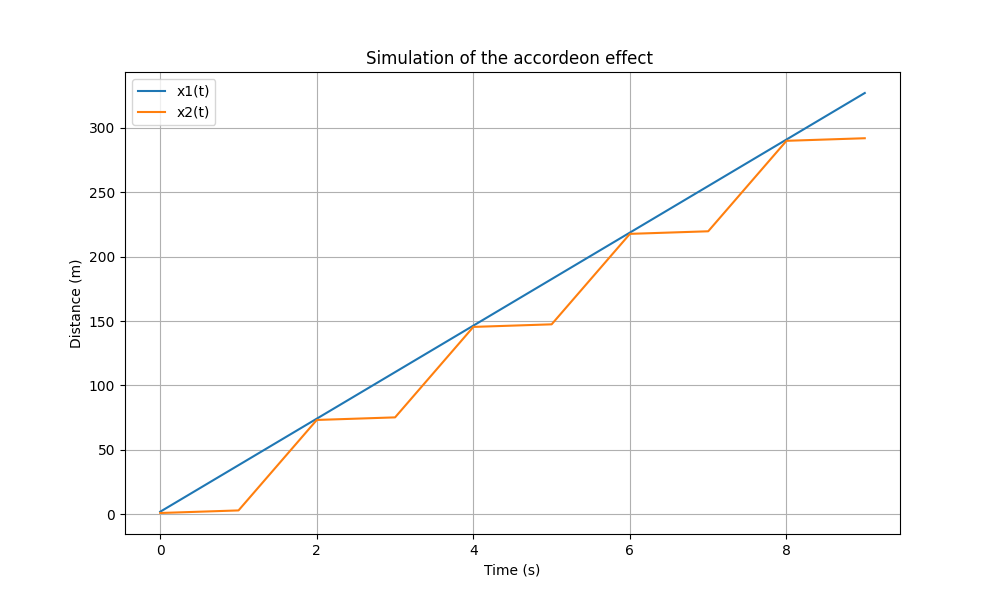
\includegraphics[width=0.8\textwidth]{Accordeon1.png}
				\caption[Simulation of accordion phenomenon]{\textbf{\underline{Simulation of accordion phenomenon : }} In this picture, you can observe the position evolutions of two cars, the first one (blue) maintaining a constant speed, and the second one (orange) following behind the first one. We could see that orange graph behaves like a periodic accordion with respect to time.}
				\label{fig:Aco1}
			\end{figure}
			
		\textbf{\underline{Simulation with the Newell's Model For Two cars}} \newline\newline
		
		Similar to the previous case, applying Newell's method yields identical results. As depicted in Figure \ref{fig:1W2_ACCORD}, the graph illustrates the accordion phenomenon, featuring distinct periods of acceleration followed by deceleration.
		
		\begin{figure}[H]
			\centering
			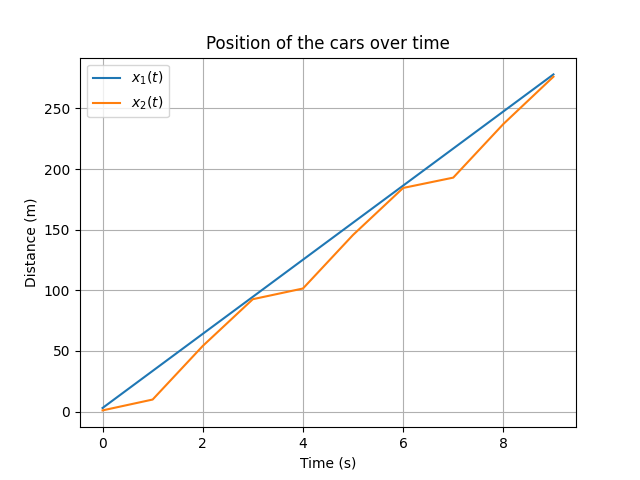
\includegraphics[width=0.8\textwidth]{1W2_Accord.png}
			\caption[Simulation of accordion phenomenon]{\textbf{\underline{Simulation of accordion phenomenon : }} In this picture, you can observe the positional evolutions of two cars. The first one (blue) maintains a constant speed, while the second one (orange) follows behind the first. It is evident that the orange graph behaves like a periodic accordion with respect to time. In the right figure, we can also see the evolutions of the car speeds, respectively represented by the same colors.}
			\label{fig:1W2_ACCORD}
		\end{figure}
		
			
		\subsubsection{Accident Phenomenon For The Linear Model }
		
		\textbf{\underline{Simulation with the Linear Model For Two cars}} \newline\newline
		
		For this case, the objectif is to show that if one driver have a bigger time reaction capacity, there is an accident.
		Onto this case, we took the same assumptions than before, but with a capacity of accelleration a little bit lower and a highter time reaction. In the algorithm \ref{alg:xi_dot} we took $\alpha_2=1.75$ and in the algorithm \ref{alg:update_positions} we took $h=1.5$
		
		On the figure \ref{fig:Acc1} accident is confirmed because there is a curve intersection (the position of the car number two (orange) is greater than the first car (blue)) So it means that the second car is crashed into the first car.
		
		\begin{figure}[H]
			\centering
			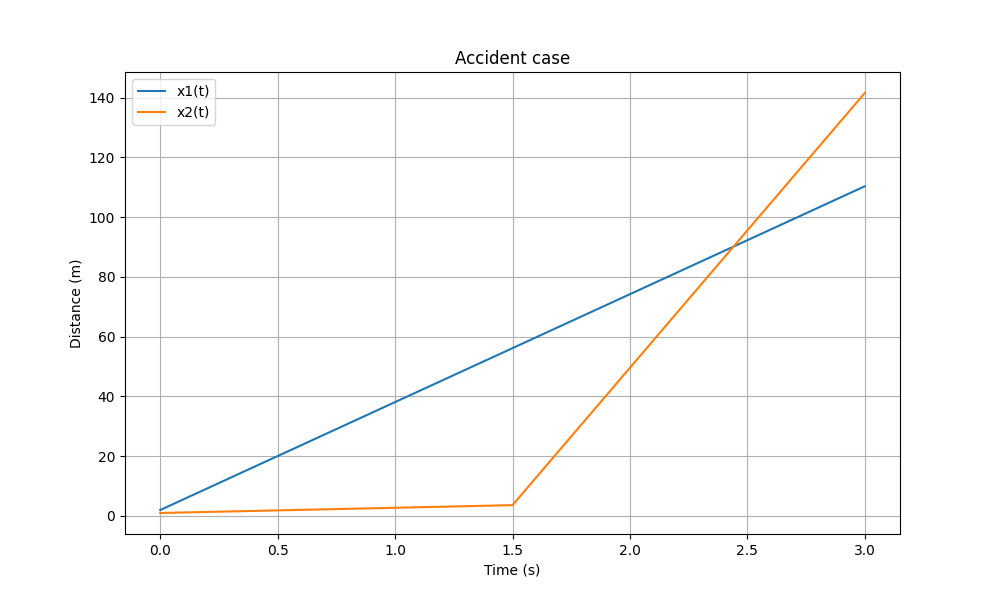
\includegraphics[width=0.8\textwidth]{Acc1.png}
			\caption[Simulation of Accident case between two cars]{\textbf{\underline{Simulation of Accident case between two cars : }} In this picture, you can observe the position evolutions of two cars, the first one (blue) maintaining a constant speed, and the second one (orange) following behind the first one. We could see on The graph shows that the acceleration of the orange car is too large. This implies an accident between two cars.}
			\label{fig:Acc1}
		\end{figure}
		
		\textbf{\underline{Simulation with the Newell's Model For Two cars}} \newline\newline
		
		In the three subsequent figures \ref{fig:1W2_ACC_1}, \ref{fig:1W2_ACC_2}, and \ref{fig:1W2_ACC_3}, we can observe a similar graph pattern to that of the linear model. However, in this scenario, we have the flexibility to vary additional parameters, such as the maximum speed of the cars (for instance, introducing a new car with a more powerful motor) and the safety distance, which is an inherent aspect of the Newell model. This variation allows us to witness accidents occurring at each curve intersection on the graph.
		
		
		\begin{figure}[H]
			\centering
			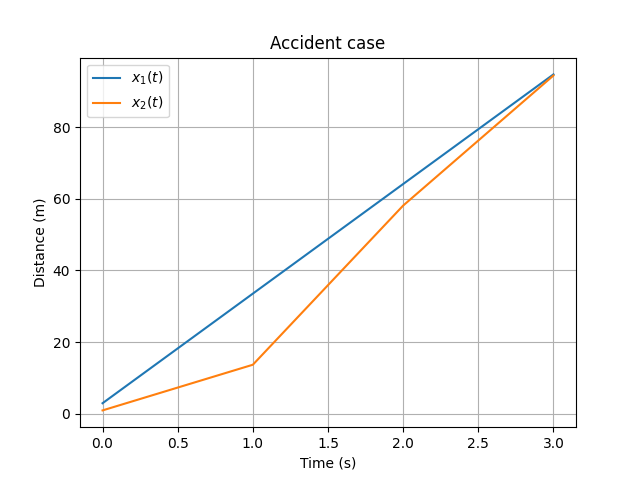
\includegraphics[width=0.5\textwidth]{1W2_Acc1.png}
			\caption[Simulation of Accident case between two cars]{\textbf{\underline{Simulation of Accident case between two cars : }} In this picture, you can observe the position evolutions of two cars, the first one (blue) maintaining a constant speed, and the second one (orange) following behind the first one. We could see on The graph shows that the acceleration of the orange car is too large. This implies an accident between two cars.}
			\label{fig:1W2_ACC_1}
		\end{figure}
		
		\begin{figure}[H]
			\centering
			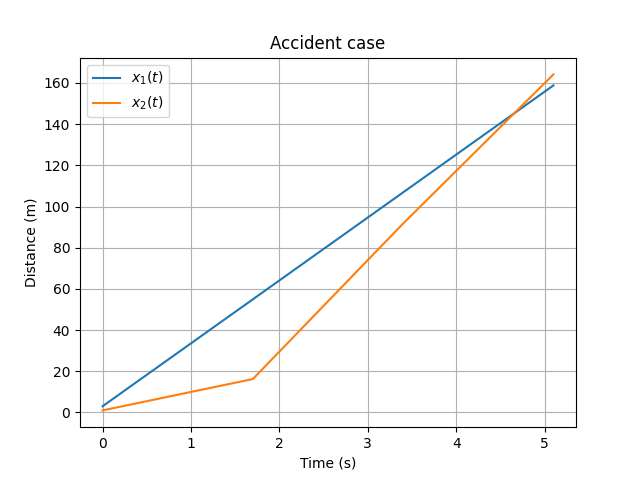
\includegraphics[width=0.5\textwidth]{1W2_Acc2.png}
			\caption[Simulation of Accident case between two cars]{\textbf{\underline{Simulation of Accident case between two cars : }} In this picture, you can observe the position evolutions of two cars, the first one (blue) maintaining a constant speed, and the second one (orange) following behind the first one. However the low reaction time of driver 2 implies an accident between two cars.}
			\label{fig:1W2_ACC_2}
		\end{figure}
		
		\begin{figure}[H]
			\centering
			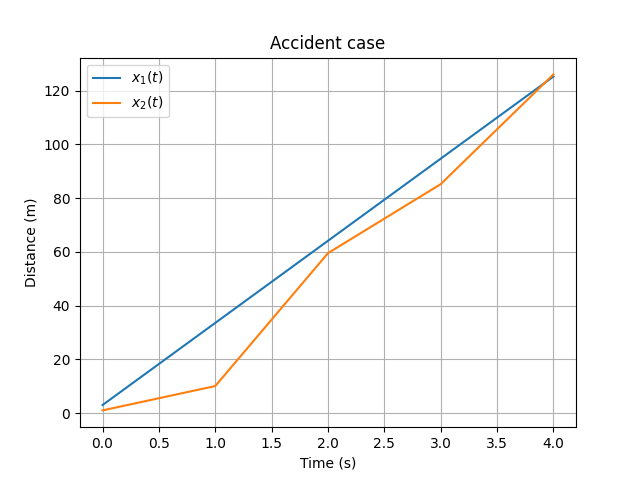
\includegraphics[width=0.5\textwidth]{1W2_Acc3.png}
			\caption[Simulation of Accident case between two cars]{\textbf{\underline{Simulation of Accident case between two cars : }} In this picture, you can observe the position evolutions of two cars, the first one (blue) maintaining a constant speed, and the second one (orange) following behind the first one. However the increasing of the maximum speed of car 2 implies an accident between two cars.}
			\label{fig:1W2_ACC_3}
		\end{figure}
		
		
		\subsection{Study of Equilibrium, Stability, and Instability of the Solution}
		\subsubsection{System Stability and Equilibrium for the Linear Model}
		In this section, the goal is to investigate the difference in distance between two cars to determine the stability of solutions and ascertain whether an equilibrium exists.
		
		To achieve this, we analyze the solutions of the following system of equations:
		\begin{align*}
			\begin{cases}
				\dot{d_1} &= V_1 - \alpha_2 \cdot d_1 \\
				&\vdots \\
				\dot{d_n} &= \alpha_n \cdot d_{n-1} - \alpha_{n+1} \cdot d_n
			\end{cases}
		\end{align*}
		
		In our context, two cars constitute a 1D system, whereas with 3 cars, we encounter a 2D system of equations.
		
		Now, let's delve into the system's stability and equilibrium:
		
		\textbf{\underline{With 2 Cars}}:
		
		The equation of interest for analysis is:
		\begin{align*}
			\dot{d_1} &= V_1 - \alpha_2 \cdot d_1
		\end{align*}
		
		Upon solving (\ref{eq:EDO1}), we obtain the following equation for \(d_1(t)\):
		\begin{align*}
			\boxed{d_1(t) = \frac{{V_1 - V_1 \cdot e^{-\alpha_2(t-t_0)} + \alpha_2 \cdot d_1(t_0) \cdot e^{-\alpha_2(t-t_0)}}}{\alpha_2}}
		\end{align*}
		
		Initially, the intuition was that if \(\alpha_2 < 0\), the solution would diverge as one car moves backward and the other forward. However, upon studying the equation, we observe that the terms \(V_1\) and \(\alpha_2 \cdot d_1(t_0)\) are constant and less significant.
		
		Nevertheless, both terms, \(e^{-\alpha_2(t-t_0)}\), represent exponential functions of time. For negative \(\alpha_2\), these exponentials grow exponentially over time.
		
		Thus, the equation is stable and converges to the equilibrium \(\boxed{d_1(t)=\frac{V_1}{\alpha_2}}\) if \(\alpha_2 > 0\).
		
		Graphically, these observations are depicted in figures \ref{fig:RC1} and \ref{fig:RS1}. Notably, across all figures, there's no occurrence of solution explosion. Specifically, in figure \ref{fig:RC1}, the car's position exhibits periodic behavior concerning time. Meanwhile, in figure \ref{fig:RS1}, the depiction illustrates the convergence of the distance between two cars towards an equilibrium state.
		
		\begin{figure}[H]
			\centering
			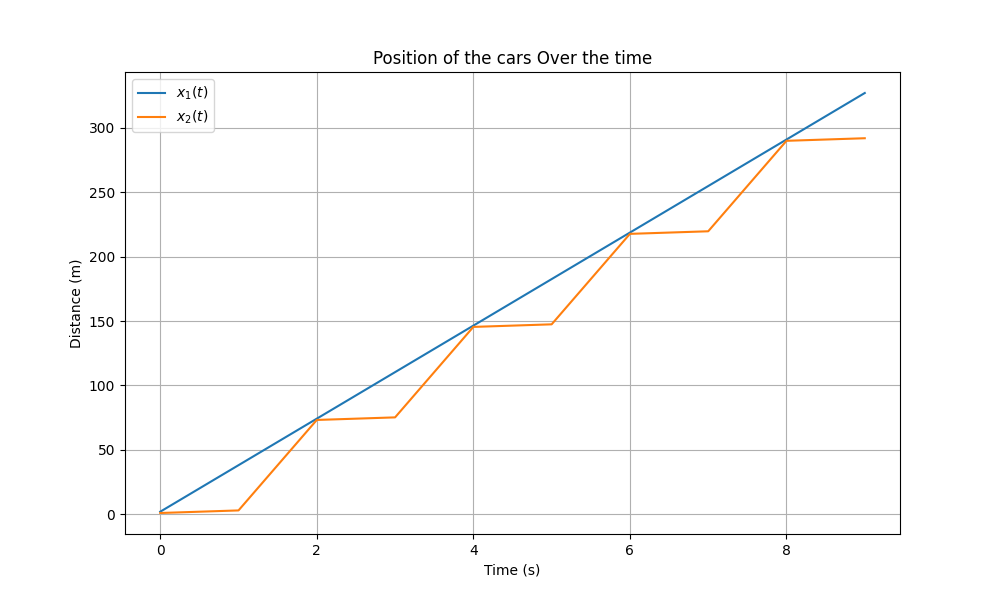
\includegraphics[width=0.8\linewidth]{RealisticCase.png}
			\caption[Realistic Case for the Linear Model with Two Cars]{\textbf{\underline{Realistic Case for the Linear Model with Two Cars: }}This simulation illustrates real-life behavior, characterized by a reaction time of approximately 1 second, achieved using a time step of 1 second instead of smaller increments in the algorithm.}
			\label{fig:RC1}
		\end{figure}
		
		\begin{figure}[H]
			\centering
			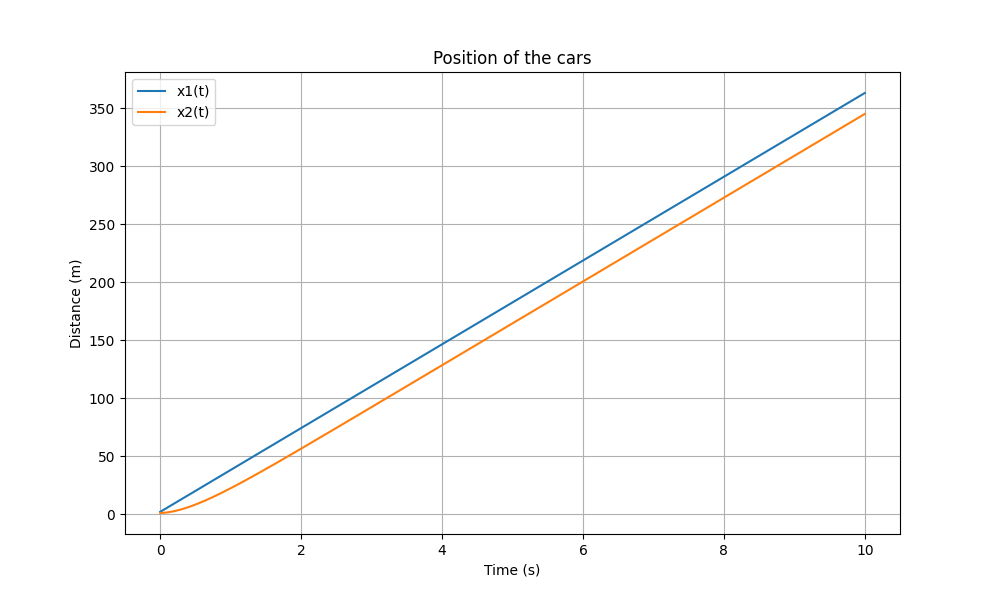
\includegraphics[width=0.8\linewidth]{RealSolCase.png}
			\caption[Real Solution for the Linear Model with Two Cars]{\textbf{\underline{Real Solution for the Linear Model with Two Cars: }}This simulation depicts the accurate solution of the ODE (Ordinary Differential Equation), portraying an infinitesimally small reaction time through the use of smaller time increments in the algorithm, rather than representing real-life scenarios.}
			\label{fig:RS1}
		\end{figure}
		
		The subsequent part of our study aims to emphasize the impact of \(\alpha_2\) values on the stability of the system. For \(\alpha_2 > 0\), the distance between two cars converges, while for \(\alpha_2 < 0\), the ODE becomes unstable.
		
		To visualize this, Figure \ref{fig:AS1} showcases different analytical solutions of the ODE with \(\alpha_2\) values greater than 0. Conversely, Figure \ref{fig:AS2} displays analytical solutions for \(\alpha_2\) values lower than 0. These plots align with theoretical predictions, demonstrating stable solutions in Figure \ref{fig:AS1}, which converge to equilibrium, while unstable solutions are evident in Figure \ref{fig:AS2}.
		
		\begin{figure}[H]
			\centering
			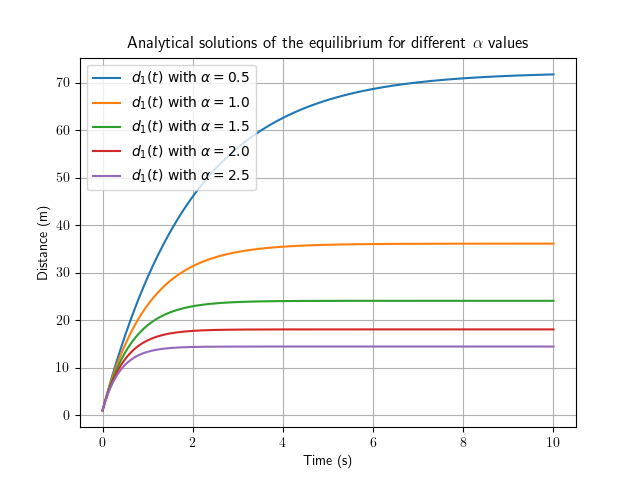
\includegraphics[width=0.8\linewidth]{Stability.png}
			\caption[Analytical Solutions for the Linear Model with Two Cars]{\textbf{\underline{Analytical Solutions for the Linear Model with Two Cars (Stability): }}Different plots displaying the Analytical Solutions for various acceleration values.}
			\label{fig:AS1}
		\end{figure}
		
		\begin{figure}[H]
			\centering
			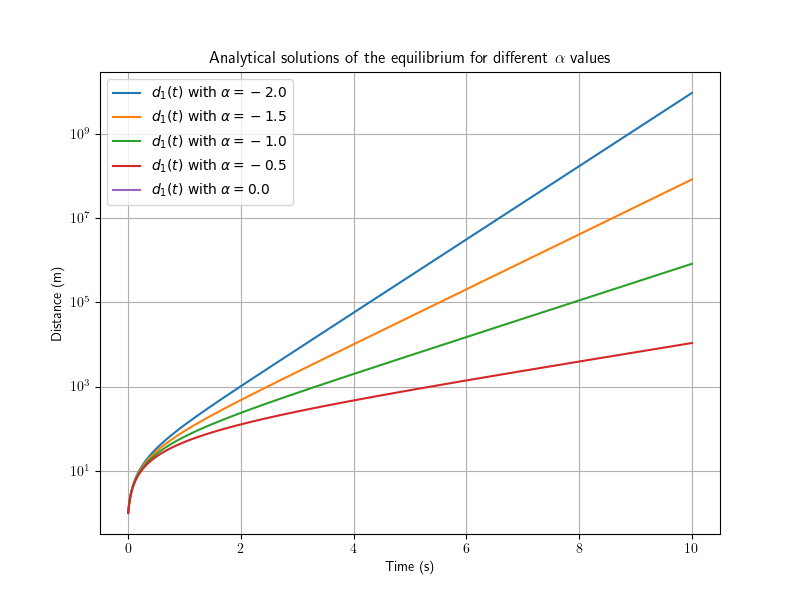
\includegraphics[width=0.8\linewidth]{Unstability.png}
			\caption[Analytical Solutions for the Linear Model with Two Cars]{\textbf{\underline{Analytical Solutions for the Linear Model with Two Cars (Instability): }}Different plots displaying the Analytical Solutions for various acceleration values.}
			\label{fig:AS2}
		\end{figure}
		
		Finally, the last step was to show how the solution behaves. On Figure \ref{fig:FV1}, for a given acceleration greater than 0, the field of vectors converges onto the equilibrium. However, for negative acceleration, the field of vectors on Figure \ref{fig:FV2} diverges from the equilibrium.
		
		\begin{figure}[H]
			\centering
			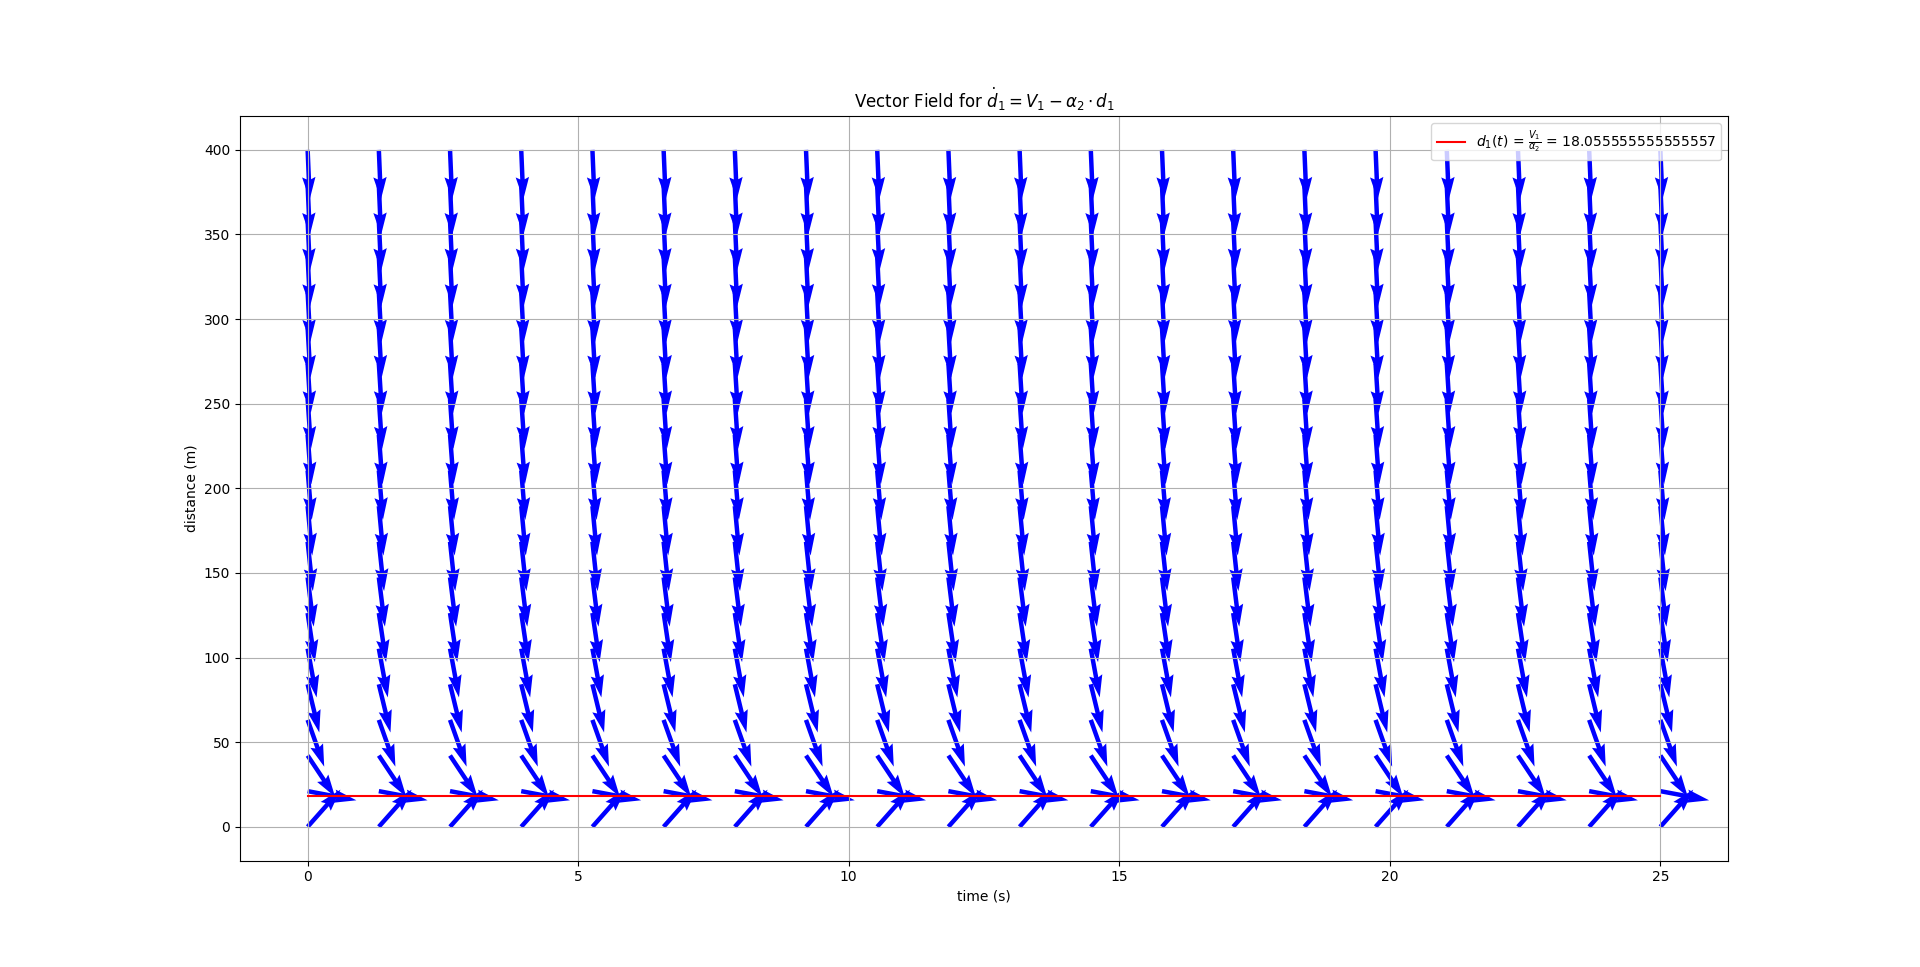
\includegraphics[width=0.8\textwidth]{FieldOfVector_CV.png}
			\caption{\textbf{\underline{Field Of Vector for the Linear Model (Stability): }} On this figure, you could see the field of vectors that converges to the equilibrium.}
			\label{fig:FV1}
		\end{figure}
		
		\begin{figure}[H]
			\centering
			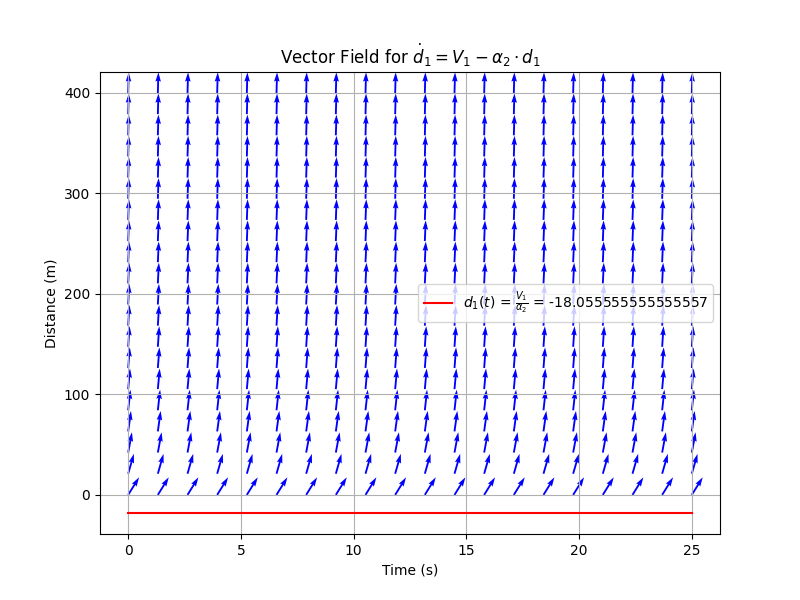
\includegraphics[width=0.8\textwidth]{FieldOfVector_DV.png}
			\caption{\textbf{\underline{Field Of Vector for the Linear Model (Instability): }} On this figure, you could see the field of vectors that diverges from the equilibrium.}
			\label{fig:FV2}
		\end{figure}
		
		\textbf{\underline{With 3 cars}} : \newline\newline
		
		After the resolution (\ref{eq:EDO2}) we obtain the next equation for $d_1(t)$ and $d_2(t)$ : 
		
		\begin{align*}
			\begin{cases}
				d_1(t) &= \frac{C_1(\alpha_3-\alpha_2)}{\alpha_2e^{\alpha_2t}}+ \frac{V_1}{\alpha_2}\\
				d_2(t) &= \frac{C_1}{e^{\alpha_2t}} + \frac{C_2}{e^{\alpha_3 \cdot t}} + \frac{V_1}{\alpha_3}
			\end{cases}
		\end{align*}
		
		we set the initial condition to $d_1(0)=m, d_2(0)=n$ So we find easily $C_1$ and $C_2$ : 
		\begin{align*}
			&C_1=\frac{m\alpha_2-V_1}{\alpha_3-\alpha_2} \\
			&C_2=n-\frac{V_1}{\alpha_3} - C_1
		\end{align*}
		
		In the scenario involving just three cars, our analysis of the formula's terms leads us to a critical observation: divergence occurs if the value of $\alpha_2$ is less than zero. This finding confirms our initial intuition. This phenomenon is rooted in the constancy of equations over time and the unchanged hypotheses, allowing us to extend this analytical process to a scenario involving 'n' cars.
		
		The visual representation in Figure \ref{fig:SE1} elucidates the equilibrium dynamics. In the left subfigure, the vector field demonstrates convergence towards the equilibrium point. Simultaneously, the right subfigure presents the Analytical Solutions derived from the system of Ordinary Differential Equations (ODEs).
		
		\begin{figure}[H]
			\centering
			\begin{subfigure}{0.45\textwidth}
				\centering
				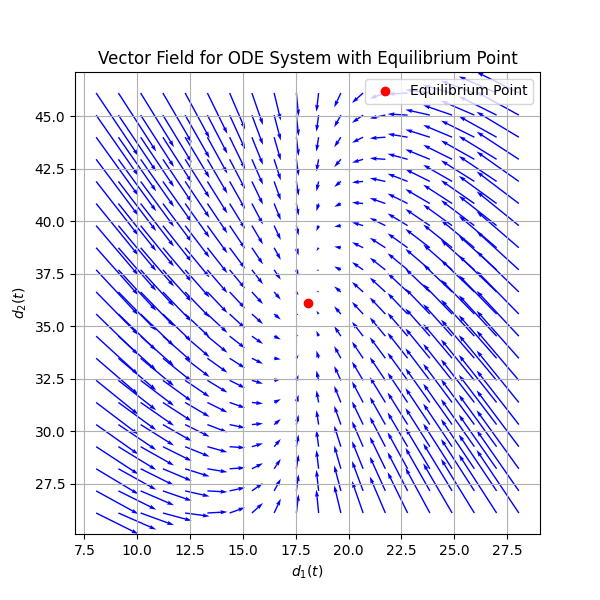
\includegraphics[width=\linewidth]{FieldOfVector_CV2.png}
			\end{subfigure}
			\hfill
			\begin{subfigure}{0.45\textwidth}
				\centering
				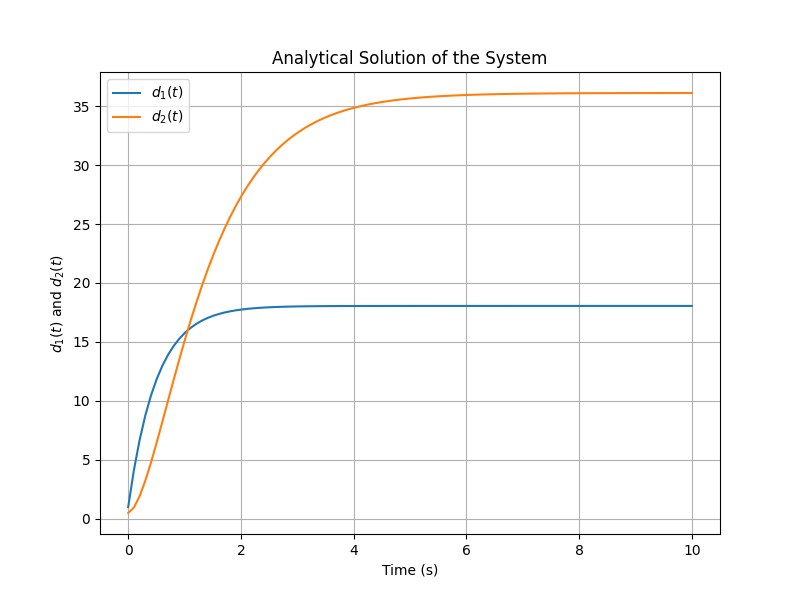
\includegraphics[width=\linewidth]{AnalyticalSolution.png}
			\end{subfigure}
			\caption{\textbf{\underline{Visualisation of the equilibrium:}} On the left figure, you could see the vector field that converges onto the equilibrium point. On the right, the Analytical Solutions of the system of ODEs.}
			\label{fig:SE1}
		\end{figure}
		
		Examining Figure \ref{fig:SE1}, it's evident that for positive acceleration, the vector field directs towards equilibrium. The distances between car 1 and 2, as well as between car 2 and 3, converge toward the equilibrium as indicated by the vector field.
		
		Contrarily, in Figure \ref{fig:SE2}, representing a scenario with negative acceleration, similar to the case of two cars, divergence is observed. Consequently, this divergence implies the absence of a feasible solution.
		
		\begin{figure}[H]
			\centering
			\begin{subfigure}{0.45\textwidth}
				\centering
				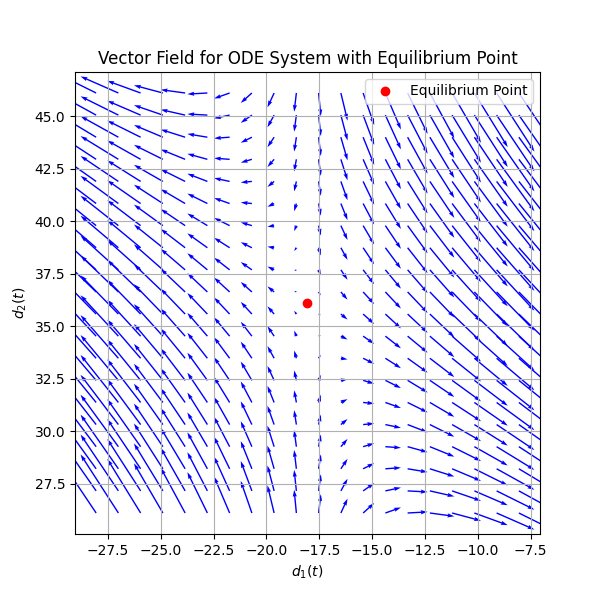
\includegraphics[width=\linewidth]{FieldOfVector_DV2.png}
			\end{subfigure}
			\hfill
			\begin{subfigure}{0.45\textwidth}
				\centering
				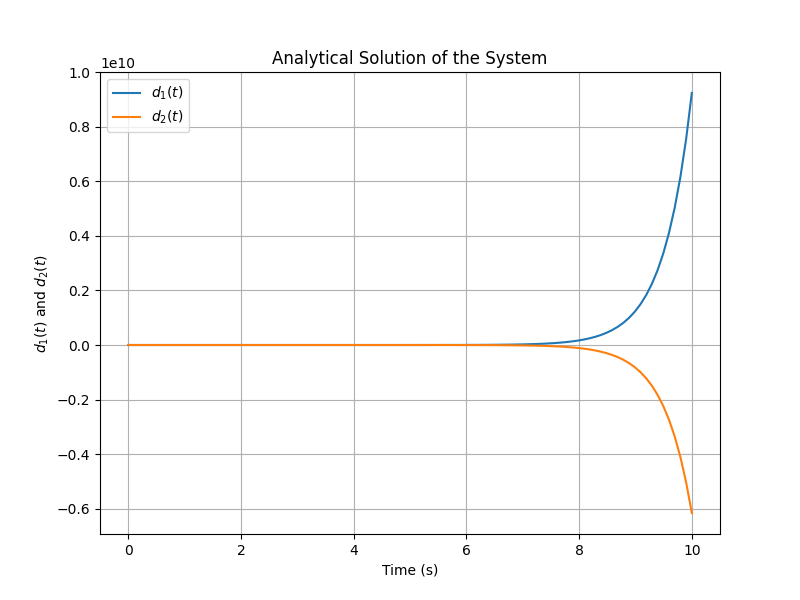
\includegraphics[width=\linewidth]{AnalyticalSolution2.png}
			\end{subfigure}
			\caption{\textbf{\underline{Visualisation of the Divergence:}} On the left figure, you could see the vector field that diverges from the theoretical equilibrium. On the right, the Analytical Solutions of the system of ODEs that completely diverge to infinity.}
			\label{fig:SE2}
		\end{figure}
		
		Figure \ref{fig:SE2} visually portrays this divergence phenomenon. The left subfigure illustrates the vector field diverging from the theoretical equilibrium point. Meanwhile, the right subfigure showcases the Analytical Solutions derived from the set of ODEs, demonstrating a complete divergence leading to infinity. This divergence pattern is consistent with the negative acceleration scenario, echoing the lack of attainable solutions, akin to the three-car case.
		
		
	\subsubsection{System Stability and Equilibrium for the Newell's Model}
	
	\textbf{\underline{The Study of the equilibrium for two cars : }} \newline\newline
	
	
	The objective here, as before, is to study the stability of the model. The 1D equation is as follows:
	
	\begin{align*}
		&\dot{d_1}(t) = \dot{x_1}(t) - \dot{x_2}(t) = V_1 - V_2 + V_2 \cdot e^{-\frac{\alpha_2}{V_2}(d_1 - d_{2}^{sec})} = f(d_1, t), \\
		&\left\{
		\begin{aligned}
			V_1 &:= \text{Maximum speed for car number 1}, \\
			V_2 &:= \text{Maximum speed for car number 2}, \\
			\alpha_2 &:= \text{capacity of acceleration for car number 2}, \\
			d_{2}^{sec} &:= \text{security distance that car number 2 maintains}.
		\end{aligned}
		\right.
	\end{align*}
	
	Firstly, let's determine the equilibrium:
	
	\begin{align*}
		V_1 - V_2 + V_2 \cdot e^{-\frac{\alpha_2}{V_2}(d_1 - d_{2}^{sec})} &= 0 \\
		e^{-\frac{\alpha_2}{V_2}(d_1 - d_{2}^{sec})} &= \frac{V_2-V_1}{V_2} \\
		e^{-\frac{\alpha_2}{V_2}d_1} &= \frac{V_2-V_1}{V_2}e^{-\frac{\alpha_2}{V_2}d_2} \\
		-\frac{\lambda_2}{V_2}d_1 &= \ln \left(\frac{V_2-V_1}{V_2}e^{-\frac{\alpha_2}{V_2}d_2} \right) \\
		d_1^* &= -\frac{V_2}{\lambda_2}\ln \left(\frac{V_2-V_1}{V_2}e^{-\frac{\alpha_2}{V_2}d_2} \right)
	\end{align*}
	
	The challenge with this equation is the inability to find an analytical solution. Consequently, we apply Lyapunov's Indirect Theorem to investigate the equilibrium.
	
	In the context of 1D analysis, we begin by calculating $f'(d_1, t)$, which results in:
	
	\[
	f'(d_1, t) = -\alpha_2e^{-\frac{\alpha_2}{V_2}(d_1 - d_{2}^{sec})}
	\]
	
	It is evident that $f'(d_1, t)$ is negative for all values of $\alpha_2$ greater than zero. Therefore, in our specific scenario, the equilibrium remains stable at all times, as negative acceleration is not considered.
	
	From the equilibrium, we also observe that the equilibrium exists if and only if $V_2 > V_1$.
	
	Clearly, the condition for a stable equilibrium is $\alpha_2 > 0$ and $V_2 > V_1$.
	

	
	\begin{figure}[H]
		\centering
		\begin{subfigure}{0.40\textwidth}
			\centering
			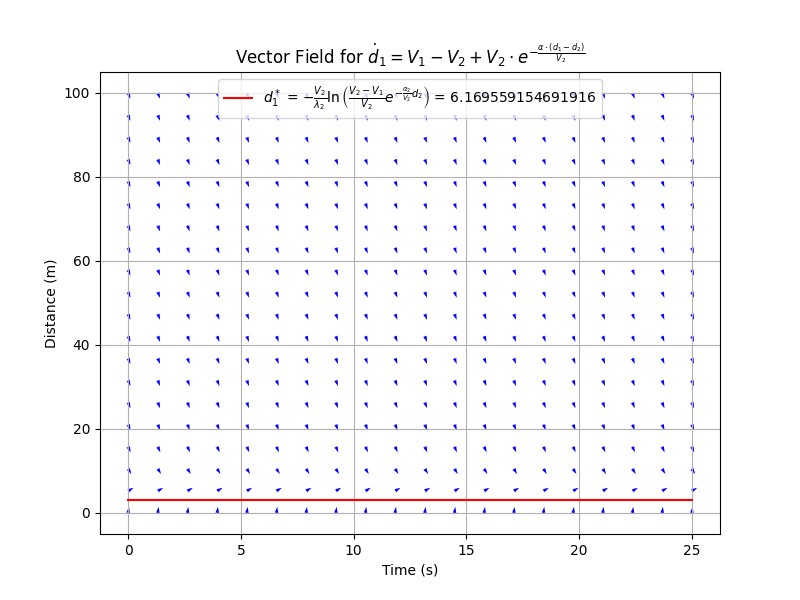
\includegraphics[width=\linewidth]{VectorFIeld.png}
		\end{subfigure}
		\hfill
		\begin{subfigure}{0.55\textwidth}
			\centering
			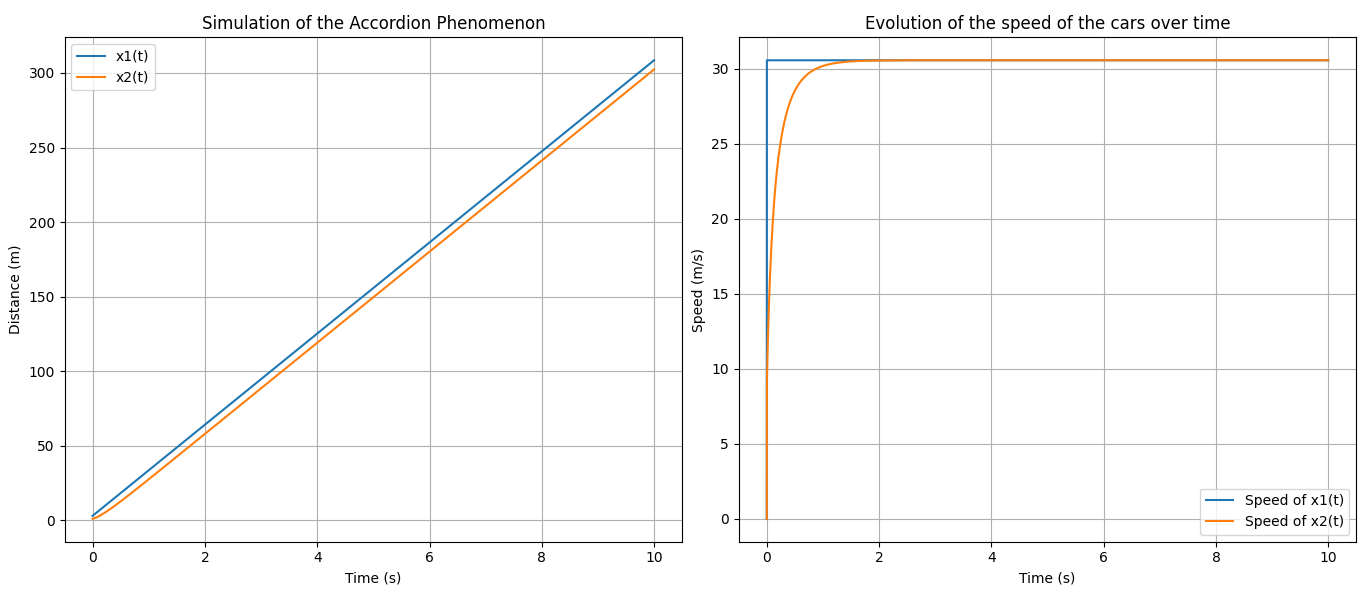
\includegraphics[width=\linewidth]{RealSol.png}
		\end{subfigure}
		\caption{\textbf{\underline{Visualisation of the equilibrium:}} On the left figure, you could see the vector field that converges onto the equilibrium point. On the right, the Approximation of the real Solutions of the system of ODEs.}
		\label{fig:SE3}
	\end{figure}
	
		Graphically, this can be observed in Figure \ref{fig:SE3}. On the left side of the figure, the phenomenon of convergence towards equilibrium can be demonstrated when the previously performed conditions are adhered to.
	
	On the right side, we depict the solutions of the system using Newell's equation. It is noticeable that over time, the distance between the two cars gradually increase at the beginning of the simulation, eventually approaching a constant value, which aligns with the equilibrium observed in the left figure.
	
	\textbf{\underline{The Study of the equilibrium for three cars : }} \newline\newline
	
	\begin{align*}
		&\begin{cases}
			\begin{aligned}
				&\dot{d_1}(t) = \dot{x_1}(t) - \dot{x_2}(t) = V_1 - V_2 + V_2 \cdot e^{-\frac{\alpha_2}{V_2}(d_1 - d_{2}^{sec})} = f(d_1, t), \\
				&\dot{d_2}(t) = \dot{x_2}(t)-\dot{x_3}(t) = V_2 - V_2 \cdot e^{-\frac{\alpha_2}{V_2}(d_1 - d_{2}^{sec})} - V_3 + V_3 \cdot e^{-\frac{\alpha_3}{V_3}(d_2 - d_{3}^{sec})}
			\end{aligned}
		\end{cases}
		 \\
		&\left\{
		\begin{aligned}
			V_1 &:= \text{Maximum speed for car number 1}, \\
			V_2 &:= \text{Maximum speed for car number 2}, \\
			\alpha_2 &:= \text{capacity of acceleration for car number 2}, \\
			d_{2}^{sec} &:= \text{security distance that car number 2 maintains}.
		\end{aligned}
		\right.
	\end{align*}
	
	again, we apply Lyapunov's Indirect Theorem to investigate the equilibrium.
	
	
	We are going to calculkate the Jacobienne matrix : 
	
	\begin{align*}
		J_{\bar{x}}=\begin{pmatrix}
			-\alpha_2e^{-\frac{\alpha_2}{V_2}(d_1 - d_{2}^{sec})} & 0 & \\
			\alpha_2e^{-\frac{\alpha_2}{V_2}(d_1 - d_{2}^{sec})} & -\alpha_3e^{-\frac{\alpha_3}{V_3}(d_2 - d_{3}^{sec})} &
		\end{pmatrix}
	\end{align*}
	
	However, in the 2D case, Lyapunov tells us that the equilibrium is stable if:
	
	\[
	\boxed{
		\begin{aligned}
			Tr(J_{\bar{x}}) &< 0 \\
			\det(J_{\bar{x}}) &> 0
		\end{aligned}
	}
	\]

	The both condition are respected iff $\lambda_2>0, \lambda_3>0$
	 \newline\newline
	 
	In the case of two cars, if the conditions are respected, we can observe graphically the convergence towards the equilibrium point. As the equations apply uniformly to all cars, the equilibrium exists under the same conditions, even for the n-th car.
	
	On the Figure \ref{fig:SE4}, the equilibrium point is represented by the coordinates corresponding to the equilibrium distance on the y-axis between car 2 and 3, and on the x-axis between car 1 and 2 on the figure \ref{fig:SE5}. This distance, similar to other cases, can be found on the figure \ref{fig:SE5} by calculating the difference between the positions of the cars.
	
	Similar to the previous scenario, the plotted solution is not the actual solution but an approximation using the Euler Explicit method because obtaining an analytical solution is impossible.
	 
	 
	 \begin{figure}[H]
	 	\centering
	 	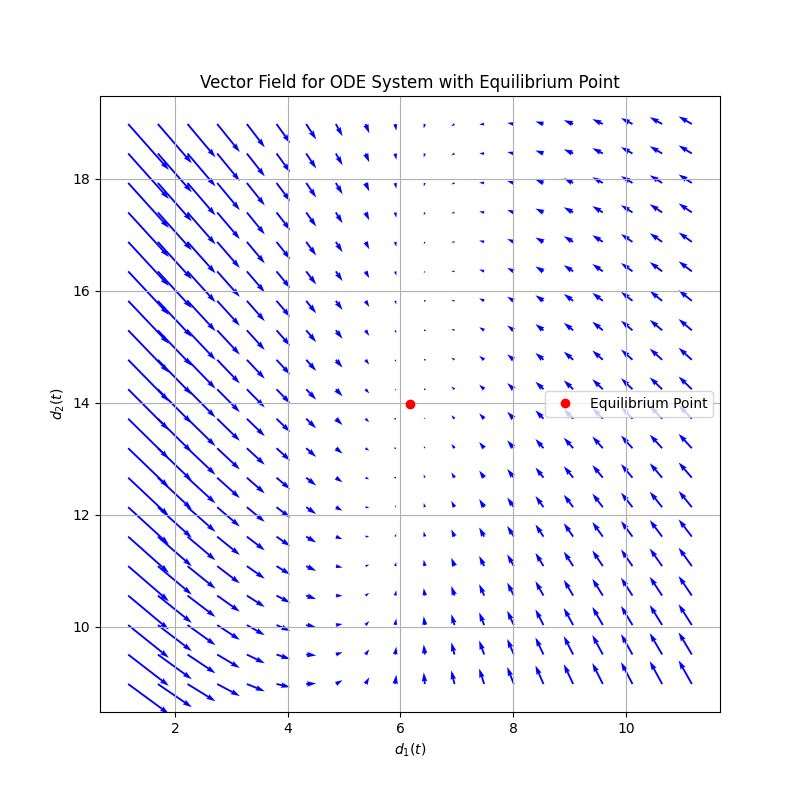
\includegraphics[width=0.5\textwidth]{VectorField1.png}
	 	\caption{\textbf{\underline{Field Of Vector for the Newell's Model (Stability): }} On this figure, you could see the field of vectors that converges from the equilibrium.}
	 	\label{fig:SE4}
	 \end{figure}
	 
	 \begin{figure}[H]
	 	\centering
	 	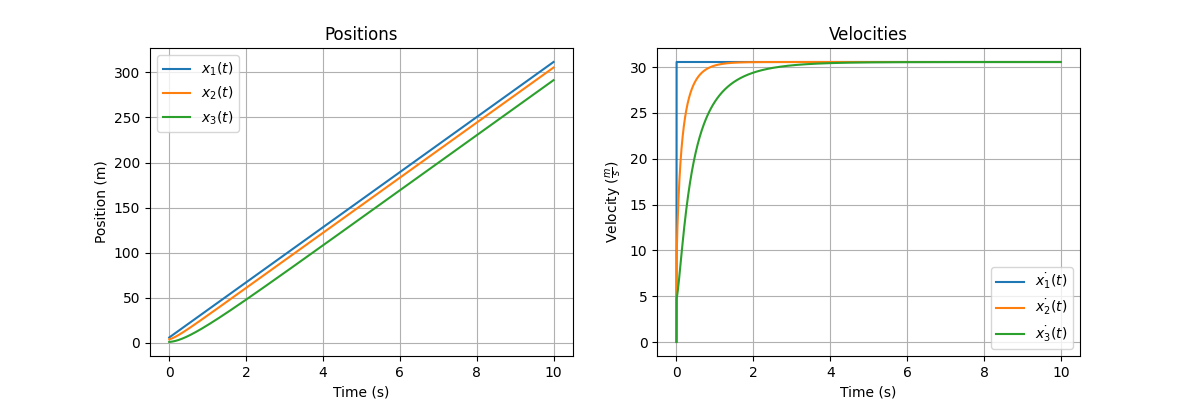
\includegraphics[width=0.8\textwidth]{RealSol1.png}
	 	\caption{\textbf{\underline{Approximation of the real solution for the Newell's Model (Stability): }} On this figure, you could see the distance between the curves that converges.}
	 	\label{fig:SE5}
	 \end{figure}
	
	
	
	\section{Types of Simulations Performed with PDE models}
	
	
	\subsection{Simulation Performed with Free Flow Model}

	
	\section{Summary}
	
	\section{Annexe}
	
	\subsection{Calculation of the Analytical solutions}
	
	\subsubsection{Linear Model for Two Cars}
	
	\label{eq:EDO1}
	\begin{align*} 
		\dot{d_1}(t) = V_1 - \alpha_2 \cdot d_1
	\end{align*}
	We use the variable separation method to Solve this EDO, so we obtain : 
	\begin{align*} 
		&\int_{x(t_0)}^{x(t_f)} \frac{1}{V_1 - \alpha_2 \cdot d_1(t)} d \ d_1(t) = \int_{t_0}^{t_f} dt \\
		&-\frac{1}{\lambda_2} \left[ \ln\left| V_1 - \alpha_2 \cdot d_1(t) \right| \right]_{x(t_0)}^{x(t_f)} = t_f-t_0 \\
		&-\frac{1}{\lambda_2} \ln\left| \frac{V_1 - \alpha_2 \cdot d_1(t_f)}{V_1 - \alpha_2 \cdot d_1(t_0)} \right| = t_f-t_0
	\end{align*}
	We could remove the |.| because the sign is always the same. And we get : 
	
	\begin{align*}
		&\ln\left( \frac{V_1 - \alpha_2 \cdot d_1(t_f)}{V_1 - \alpha_2 \cdot d_1(t_0)} \right)  = -\lambda_2( t_f-t_0)\\
		&\frac{V_1 - \alpha_2 \cdot d_1(t_f)}{V_1 - \alpha_2 \cdot d_1(t_0)}  = e^{-\lambda_2( t_f-t_0)} \\
		&V_1 - \alpha_2 \cdot d_1(t_f)   = (V_1 - \alpha_2 \cdot d_1(t_0))e^{-\lambda_2( t_f-t_0)} \\
		&\boxed{
			d_1(t) = \frac{V_1 - [V_1 - \alpha_2 \cdot d_1(t_0)]e^{-\lambda_2( t_f-t_0)}}{\alpha_2}
		}
	\end{align*}

	\subsubsection{Linear Model for Three Cars}
	\label{eq:EDO2}
	The system under matricial form coul be write like that :
	
	\begin{align*}
		\dot{D}=(t)\begin{pmatrix}
			-\alpha_2 & 0 \\
			\alpha_2 & -\alpha_3
		\end{pmatrix}
		\begin{pmatrix}
			d_1 \\
			d_2
		\end{pmatrix} + 
		\begin{pmatrix}
			V_1 \\
			0
		\end{pmatrix}
	\end{align*}
	
	The first step is to perfom the eigenvectors of the matrix:
	
	\begin{align*}
		\begin{vmatrix}
			X+\alpha_2 & 0 \\
			\alpha_2 & X+\alpha_3
		\end{vmatrix} = (X+\alpha_2)(X+\alpha_3=X^2+X(\alpha_3+\alpha_2)+\alpha_2\alpha_3
	\end{align*}
	by simple resolution of the second order polynomial, we could fin two eigenvalues: \newline
	$\lambda_1=-\alpha_2, \lambda_2 = -\alpha_3$
	we looking for the two eigen vectors : 
	
	\[
	\begin{cases}
		\begin{bmatrix}
			0 & 0 & | & 0 \\
			\alpha_2 & -\alpha_3 + \alpha_2 & | & 0
		\end{bmatrix} \\ \\
		\begin{bmatrix}
			-\alpha_2 + \alpha_3 & 0 & | & 0 \\
			\alpha_2 & 0 & | & 0
		\end{bmatrix}
	\end{cases}
	\]
	
	It is easy to see that the two following vector are vector that verify the condition : 
	
	\[
	\begin{cases}
		u_1=\begin{pmatrix}
			1 \\
			\frac{\alpha_3-\alpha_2}{\alpha_2}
		\end{pmatrix} \\ \\
		u_2=\begin{pmatrix}
			0 \\
			1
		\end{pmatrix}
	\end{cases}
	\]
	
	Then, we know that a general solution of the equation is : 
	\begin{align*}
		&\bar{D}
		(t) = \sum_{i=1}^2 X_i \\
		&\text{where } X_i = C_i e^{\lambda_it} u_i, \\
		&\text{with } C_i \text{ being constants to be determined, and } u_i \text{ as the eigenvectors}, \textbf{and} \lambda_i \textbf{the eigenvalues}.
	\end{align*}
	
	So : 
	\begin{align*}
		X_1=\begin{pmatrix}
			\frac{C_1(\alpha_3-\alpha_2)}{\alpha_2e^{\alpha_2t}} \\ \\
			\frac{C_1}{e^{\alpha_2t}}
		\end{pmatrix} \\ \\ 
		X_2=\begin{pmatrix}
			0 \\
			\frac{C_2}{e^{\alpha_3 \cdot t}}
		\end{pmatrix}
	\end{align*}
	
	Finally the general solution is given by : 
	
	\begin{align*}
		\bar{X}
		=\begin{pmatrix}
			\frac{C_1(\alpha_3-\alpha_2)}{\alpha_2e^{\alpha_2t}} \\ \\
			\frac{C_1}{e^{\alpha_2t}} + \frac{C_2}{e^{\alpha_3 \cdot t}}
		\end{pmatrix} \\ \\ 
	\end{align*}
	
	Then we are going to find for particular solution : 
	
	
	\begin{align*}
		\begin{cases}
			\dot{d_1} &= 0 \\
			\dot{d_2} &= 0
		\end{cases} \iff 
		\begin{cases}
			d_1^* &= \frac{V_1}{\alpha_2} \\
			d_2^* &= \frac{V_1}{\alpha_3}
		\end{cases}
	\end{align*}
	
	In clear, we have : 
	\begin{align*}
		\begin{cases}
			d_1(t) &= \frac{C_1(\alpha_3-\alpha_2)}{\alpha_2e^{\alpha_2t}}+ \frac{V_1}{\alpha_2}\\
			d_2(t) &= \frac{C_1}{e^{\alpha_2t}} + \frac{C_2}{e^{\alpha_3 \cdot t}} + \frac{V_1}{\alpha_3}
		\end{cases}
	\end{align*}
	
	we set the initial condition to \newline 
	$d_1(0)=m, d_2(0)=n$ So we find easily $C_1 and C_2$ : 
	\begin{align*}
		&C_1=\frac{m\alpha_2-V_1}{\alpha_3-\alpha_2} \\
		&C_2=n-\frac{V_1}{\alpha_3} - C_1
	\end{align*}
	
	\newpage
	
	%\bibliographystyle{plain}
	\printbibliography
	%\bibliography{Rapport}
\end{document}